\documentclass[conference]{IEEEtran}
\IEEEoverridecommandlockouts
% The preceding line is only needed to identify funding in the first footnote. If that is unneeded, please comment it out.
\usepackage{cite}
\usepackage{amsmath,amssymb,amsfonts}
\usepackage{algorithmic}
\usepackage{algorithm}
\usepackage{graphicx}
\usepackage{textcomp}
\usepackage{xcolor}
\def\BibTeX{{\rm B\kern-.05em{\sc i\kern-.025em b}\kern-.08em
    T\kern-.1667em\lower.7ex\hbox{E}\kern-.125emX}}
\begin{document}

\title{PAIRT: Accurate identification pipeline helping for Real time PCR\\
}

\author{\IEEEauthorblockN{Doan Vu Thinh}
\IEEEauthorblockA{\textit{Faculty of Information Technology} \\
\textit{Nha Trang University}\\
Khanh Hoa, Viet Nam \\
thinhdv@ntu.edu.vn}
}
\maketitle

\begin{abstract}
PairT (Pipeline for Analysis of Next-generation sequencing Data in Linux) is a tool for accurate identification helping for Real Time PCR  from medium to large sized haploid next-generation re-sequencing (NGS) datasets. The input requires paired-end data from the Illumina MiSeq, HiSeq platforms. PairT is an analysis pipeline with a user-friendly and it integrates the following validated bioinfor-matics tools for start-to-finish sequence analysis of raw NGS data using a single command.  The pipeline, written in BASH, uses data reduction techniques and other stand alone software packages to perform quality trimming and adapter removal, read mapping, BED coverage analyzing. The pipeline and a comprehensive user guide can be found at https://github.com/thinhdoanvu/PairT/tree/master/Source.
\end{abstract}

\begin{IEEEkeywords}
PairT, Next Genene, presence absence analysis, coverage Bedtools.
\end{IEEEkeywords}

\section{Introduction}
Next-generation sequencing (NGS) has transformed the field of genetics into genomics by providing DNA se-quence data at an ever increasing rate and reduced cost \cite{ER2008}. Three platforms for massively parallel DNA sequencing read production are in reasonably widespread use at present: the Roche/454 (http://www.454.com), the Illumina/Solexa (http://www.illumina.com), and SOLiDTM System (http://marketing.appliedbiosystems.com).

The Burkholderia genus contains over 60 species and occupies a large range of environments including soil, plants, rhizospheres, water, animals and humans \cite{Ginther2015}. The identification of novel species in new loca-tions necessitates the need to identify the true global distribution of Burkholderia species, especially the members that are closely related to B. pseudomallei. Burkholderia ubonensis - whole genome shotgun sequence can be found at GenBank by ID ABBE01000101.1 (https://www.ncbi.nlm.nih.gov/nuccore/ABBE01000101.1).

Over 500 thousands reads for each forward and reverse sequence files, need to have pipeline to process huge data and to take full advantage of high performance PC. Here, the pipeline PairT is introduced as a tool for accurate identification helping for Real Time PCR genomic data; PairT is a wrapper script designed to take raw data, taking full advantage of both paired-end reads. As input, PairT takes paired FASTQ files for individuals and outputs show the percentage of reads which overlap through all pairs. The pipeline and a comprehensive online manual can be found at https://github.com/thinhdoanvu/PairT.

\section{Methods}

\subsection{Implementation and basic usage}

The PairT pipeline is written in BASH and will run using most Unix-like operating systems through largely de-pendent on other bioinformatics software packages. Proper implementation depends on the correct installation of each third-party packages/tools. A full list of dependencies can be found at (https://github.com/thinhdoanvu/PairT/requires.sh) and a sample script to automatically download and install the packages in a Linux environment can be found at the PairT repository (https://github.com/thinhdoanvu/PairT).

PairT is run by simply switching to a directory containing input data and starting the program. The program can be run with or no need configuration file, and PairT will proceed through a short series of command line prompts, al-lowing the user to establish analysis parameters. Whole genome shotgun sequence can be found at GenBank by ID ABBE01000101.1 (https://www.ncbi.nlm.nih.gov/nuccore/ABBE01000101.1)

\section{Data input requirements}
airT requires both compressed forward and reverse FASTQ files for each individual in the analysis. A simple naming convention (a single-word locality code/name and a single-word sample identifier separated by an underscore) must be followed for every sample; examples are LOCAL\textunderscore IND01.F.fastq.gz and LOCAL\textunderscore IND01.R.fastq.gz. A sam-ple script for naming convention, can be found at the github repository (https://github.com/thinhdoanvu/PairT/rename4PairT.sh.

\subsection{Quality trimming}
Once the sequencing is finished, the data are stored in a "fastq" text files, in which each short read takes up four lines. The first line (starting with an @) is a read identifier, the second is the DNA sequence, the third another identifier (same as line 1, but starting with a +(or sometimes only consisting of a +)) and the fourth is a Phred quality score sym-bol for each base in the read. The quality score is based on the ASCII character code used by computer keyboards (http://www.ascii-code.com/). Illumina's current sequencing pipeline (as of January 2012) uses an offset of 64, so that an @ (ASCII code 64) is 0, and h (ASCII code 104) is 40 (other versions of the pipeline might use different offsets, however. The quality score for each base ranges from -5 to 40 and is defined as Qphred =-10 log10(p), where p is the estimated probability of a base call being wrong. So a Qphred of 20 corresponds to a 99\% probability of a correctly identified base. When working with high-throughput sequencing data, the quality of raw reads will need to assess using the Phred Quality Score by FASTQC tool (http://www.bioinformatics.babraham.ac.uk/projects/fastqc). PairT can use the program fastp [1] to simultaneously remove Illumina adapter sequences and trim ends of reads of low quality. By default, fastp trims bases with quality scores less than PHRED 10 (corresponding to a 10\% chance of error in the base call).

\subsection{Read maping}
PairT uses the MEM algorithm \cite{Li2013} of BWA \cite{Li2010},\cite{Li2009} to map quality-trimmed reads to the reference contigs. Two options can be uesed for maping reads with reference, the default values or set an alternative value for each mapping parameter (match score - optA, mismatch score-optB, and gap-opening penalty-optO). The default settings are meant for mapping reads to the human genome, so users are encouraged to experiment with mapping parameters. BWA output is ported to SAMtools \cite{Li2009a}, saving disk space, and alignments are saved to the disk as binary alignment/Map (BAM). BAM files are then sorted and indexed.

\subsection{Locus presence/absence analysis}
First, quality-trimmed forward and reverse reads are reduced to unique reads. This data set is then mapped to all reference sequences, using the previously entered mapping settings. From this alignment, a set of intervals is created using BEDtools \cite{Quinlan2010}. The coverageBed module of BEDTools was used for presence/absence analy-sis based on a 1 kb window size. Candidate B. ubonensis specific loci were identified by locating regions with 100\% read coverage was chosen for real-time PCR assay design following confirmation of in silico specificity for B. ubonen-sis using Microbial Nucleotide BLAST. PairT provides a combined BEDcov matrix for all analysed genomes in Bed-cov\textunderscore merge.txt. This file lists the BEDTools ‘windows’, or NGS read coverage, for each strain based on the reference sequence, and ranges from 0 (0\% read coverage across the window) to 1 (100\% coverage across the window). The BEDcov matrix can be imported into Microsoft Excel for easier visualisation and manipulation.
\section{RESULTS AND DISCUSSION}
\subsection{Quality trimming}
Over 1 million raw reads with 36 million bases are discovered from B. ubonensis individuals, are presented in Table 1  Detail information can be shown in Figure 1. Quality score across bases, Quality per tile, and GC distribution over all sequences. First, fastp seeks the overlap of each pair and considers the bases that fall out of the overlapped regions as adapter contents. There are 4 adapters remain in 4 sequence file. There are, GCCTGATGCG,  GCTG-GAAAAA, GCTGGAAAAA, and TGCGCTGGTG in REL\textunderscore 217,  REL\textunderscore 607 sequences, respectively. Second, fastp only corrects a mismatched base pair with an imbalanced quality score. Totally, 16,541,839 bases (827337-read1, and 8268468-read2), and 16,002,239 bases (8000197-read1, and 8002042-read2) for REL\textunderscore 217, REL\textunderscore 607 individuals, respectively.  PairT saves all results in trim\textunderscore report folder, and all information can be found in log files.
\subsection{Read maping and Locus presence/absence analysis}
Mapping is to create an alignment file also known as a Sequence/Alignment Map (SAM) file for each of your samples. This SAM file will contain one line for each of the reads in your sample denoting the reference sequence (genes, contigs, or gene regions) to which it maps, the position in the reference sequence (Table 2), and a Phred-scaled quality score of the mapping, among other details. Matching reference genome to which the reads align are presented from IGV [8] in Figure 2. Finaly, 17 candidates loci with 100\% coverage on both samples were chosen for real-time PCR (Table 3). There are 228 loci with 100\% are discorved on REL\textunderscore 217 individual, compare with 211 loci are shown on REL\textunderscore 607 individual.
\begin{table}[htbp]
	\caption{Raw reads information}
	\begin{center}
		\begin{tabular}{|c|l|}
			\hline
			\textbf{Sequence} & \textbf{Information}\\
			\hline
			{REL\textunderscore 217.F.fastq.gz}
			&reads: 250,000\\
			&len: 36\\
			&len mean: 36.0000\\
			&len stdev: 0.0000\\
			&len min:	36\\
			&phred: 33\\
			&\%GC: 48.3835\\
			&\%N: 0.0007\\
			&total bases: 9,000,000\\
			\hline
			{REL\textunderscore 217.R.fastq.gz}
			&reads: 250,000\\
			&len: 36\\
			&len mean: 36.0000\\
			&len stdev: 0.0000\\
			&len min: 36\\
			&phred: 33\\
			&\%GC: 49.1577\\
			&\%N: 0.0026\\
			&total bases: 9,000,000\\
			\hline
			{REL\textunderscore 607.F.fastq.gz}
			&reads: 250,000\\
			&len: 36\\
			&len mean: 36.0000\\
			&len stdev: 0.0000\\
			&len min: 36\\
			&phred: 33\\
			&\%GC: 48.1350\\
			&\%N: 0.0005\\
			&total bases: 9,000,000\\
			\hline
			{REL\textunderscore 607.R.fastq.gz}
			&reads: 250,000\\
			&len: 36\\
			&len mean: 36.0000\\
			&len stdev: 0.0000\\
			&len min: 36\\
			&phred: 33\\
			&\%GC: 48.7542\\
			&\%N: 0.0065\\
			&total bases: 9,000,000\\
			\hline
			\multicolumn{2}{l}{$^{\mathrm{}}$Note: \%GC is the percentage of nitrogenous bases in a DNA}\\
			\multicolumn{2}{l}{$^{\mathrm{}}$or RNA molecule that are either guanine (G) or cytosine (C).}
		\end{tabular}
	\end{center}
\end{table}
\begin{figure}[htbp]
	\centerline{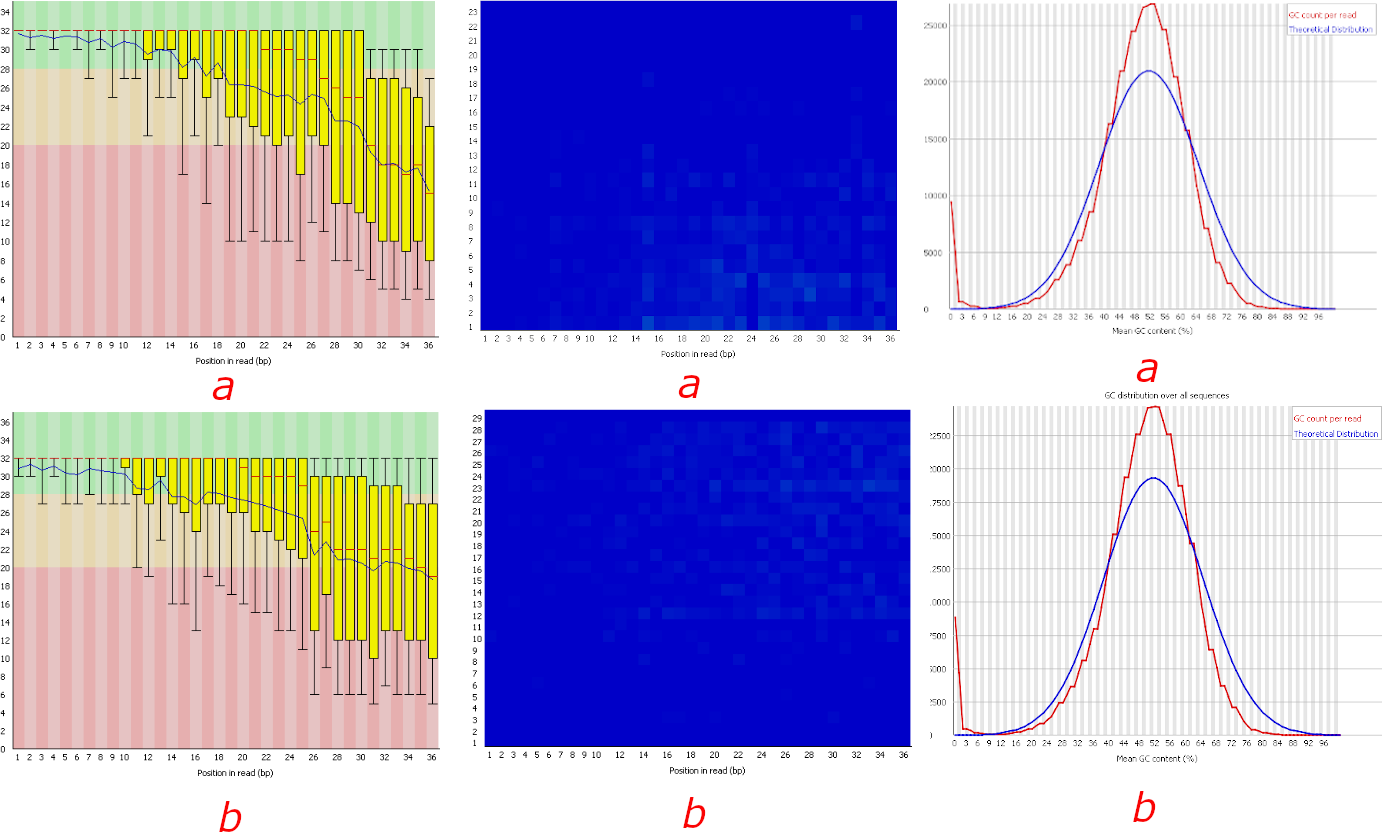
\includegraphics[scale = 0.8]{Fig1.png}}
	\caption{Quality score across bases, Quality per tile, and GC distribution over all sequences (Before (a) and After (b) trimming).}
	\label{fig}
\end{figure}
\begin{table}[htbp]
	\caption{Reference reads information}
	\begin{center}
		\begin{tabular}{|c|l|}
			\hline
			\textbf{Sequence} & \textbf{Information}\\
			\hline
			{reference.fasta}&reads: 1\\
			&len: 4,629,811\\
			&len mean: 4,629,811.0000\\
			&len min:	4,629,811\\
			&phred: 64\\
			&qual min: 40\\
			&qual max: 40\\
			&qual mean: 40.0000\\
			&qual stdev: 0.0000\\
			&\%GC: 42.8571\\
			&\%N: 0.0000\\
			&total bases: 4,629,811\\
			\hline
			\multicolumn{2}{l}{$^{\mathrm{}}$Note: \%GC is the percentage of nitrogenous bases in a DNA}\\
			\multicolumn{2}{l}{$^{\mathrm{}}$or RNA molecule that are either guanine (G) or cytosine (C).}
		\end{tabular}
	\end{center}
\end{table}
\begin{figure}[htbp]
	\centerline{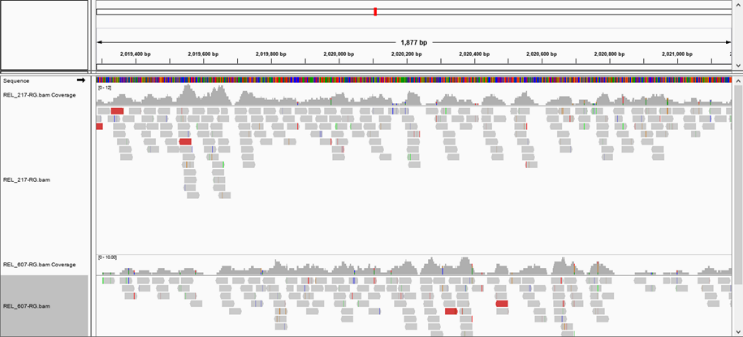
\includegraphics[scale = 1]{Fig2.png}}
	\caption{Visualize sequence read alignment data (BAM or SAM) on IGV}
	\label{fig}
\end{figure}
\begin{table}[htbp]
	\caption{BEDcov result for all \textit B. ubonensis}
	\begin{center}
		\begin{tabular}{|c|c|c|c|c|}
			\hline
			\textbf{Chrom} & \textbf{Start} & \textbf{End} & \textbf{REL\textunderscore 217} & \textbf{REL\textunderscore 607}\\
			\hline
			{NC\textunderscore 012967} & {44245} & {44389} & {1} & {1}\\
			\hline
			{NC\textunderscore 012967} & {73992} & {74246} & {1} & {1}\\
			\hline
			{NC\textunderscore 012967} & {711607} & {711691} & {1} & {1}\\
			\hline
			{NC\textunderscore 012967} & {882775} & {884689} & {1} & {1}\\
			\hline
			{NC\textunderscore 012967} & {896465} & {896824} & {1} & {1}\\
			\hline
			{NC\textunderscore 012967} & {1021806} & {1021936} & {1} & {1}\\
			\hline
			{NC\textunderscore 012967} & {1236839} & {1236934} & {1} & {1}\\
			\hline
			{NC\textunderscore 012967} & {1425132} & {1425188} & {1} & {1}\\
			\hline
			{NC\textunderscore 012967} & {2084572} & {2084697} & {1} & {1}\\
			\hline
			{NC\textunderscore 012967} & {2273956} & {2274553} & {1} & {1}\\
			\hline
			{NC\textunderscore 012967} & {3123762} & {3123918} & {1} & {1}\\
			\hline
			{NC\textunderscore 012967} & {3245321} & {3246619} & {1} & {1}\\
			\hline
			{NC\textunderscore 012967} & {3299370} & {3299462} & {1} & {1}\\
			\hline
			{NC\textunderscore 012967} & {3941651} & {3942049} & {1} & {1}\\
			\hline
			{NC\textunderscore 012967} & {4164478} & {4164555} & {1} & {1}\\
			\hline
			{NC\textunderscore 012967} & {4265853} & {4266908} & {1} & {1}\\
			\hline			
			{NC\textunderscore 012967} & {4464049} & {4464124} & {1} & {1}\\
			\hline
		\end{tabular}
	\end{center}
\end{table}
\begin{figure}[htbp]
	\centerline{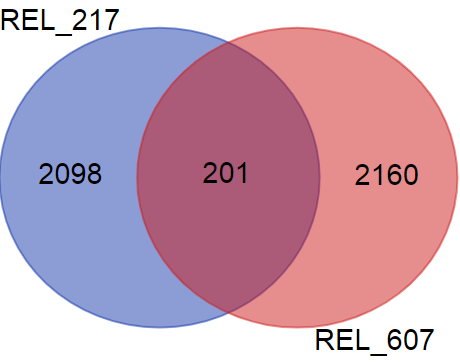
\includegraphics[scale = 0.5]{Fig3.png}}
	\caption{Venn diagram for all candidate loci on both individuals REL \textunderscore 207 and REL\textunderscore 617}
	\label{fig}
\end{figure}
\subsection{Conclusion}
PairT is an open-source, freely available genomics pipeline configured for species with NGS data. The PairT pi-peline and a comprehensive online manual can be found at (https://github.com/thinhdoanvu/PairT/tree/master/Source).
\section*{Acknowledgment}
I would like to thank Le Thanh Cuong - PhD Student at Sunshine Coast University, Queensland, Australia for assistance data in beta testing. I also would like to thank the reviewers for their substantial help with troubleshooting.
\bibliography{ICT2019_Paper20.bib}
\bibliographystyle{ieeetr}
\vspace{12pt}
\color{red}
\end{document}
